\section{Physical layer}
\label{physical}

This layer is about physical properties of the hardware and the signal itself.
In this section these properties will be analysed through the aid of various experiments performed on the prototype system.
%motivation
This is a first step in understanding the potential and the limitations of a system, because whatever limitation derives from the physical layer, it will be a hard limitation that will affect the entire system.
Therefore, starting to look at physical constraints of the system will give a good overview of what can be achieved and what cannot early on, before the rest of the designing process.
The end goal of the system will be to achieve communicatoin rates above 65 Hz, and allowing a receiver to localise the light source.
To allow this, the physical layer of the system needs to allow a light to turn on in less than 15 ms, and the light to be visible within a range.
% experimental setup
All the following experiments will be performed on the prototype system as described in section \ref{expsetup}, with the use of the low power 10mm LED unless otherwise stated.
%why brigthness in %
A remark on the experiments that will follow is that brightness will be always reported in percentage.
This serves the purpose of making the data applicable in general cases, even with different light sources and different sensors.
The LED used for testing produces a luminous intensity of about 8 000 to 10 000 MCD at 25$^{\circ}$ Celsius \cite{ledDS}.

%warmup
\subsection{Warmup time}

%These are stats for warmup only at dark
\begin{figure}[h]
\centering
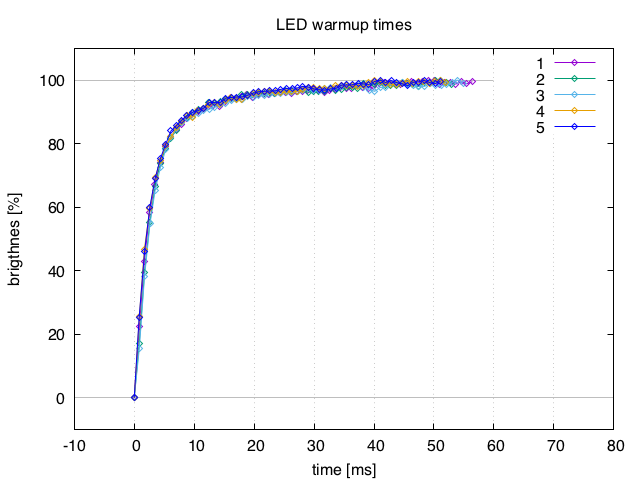
\includegraphics[height=140px]{img/warmup1}
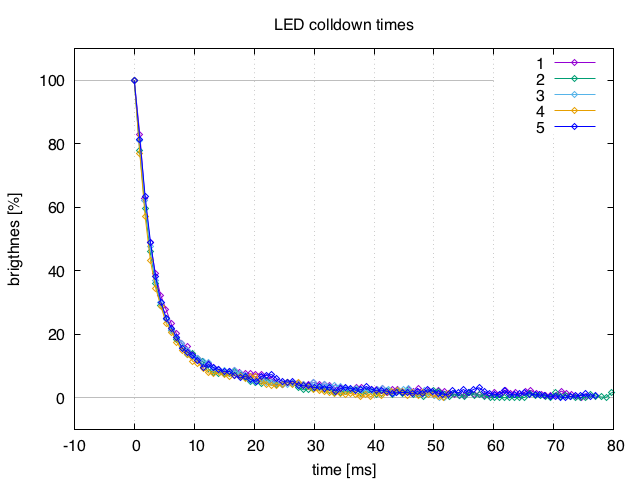
\includegraphics[height=140px]{img/warmdown1}
\caption{LED warmup and cooldown times.}
\label{fig:warmup}
\end{figure}

\begin{figure}[hbt]
\centering
  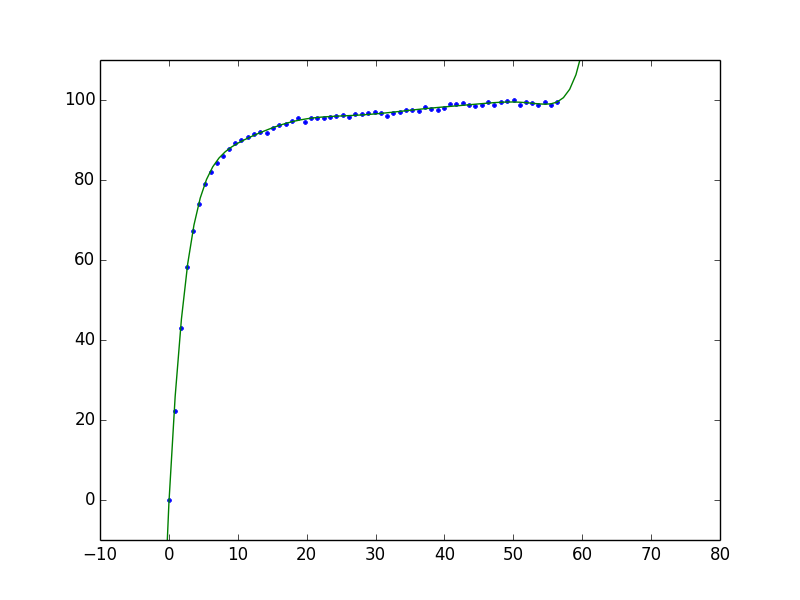
\includegraphics[height=140px]{img/regrU}
    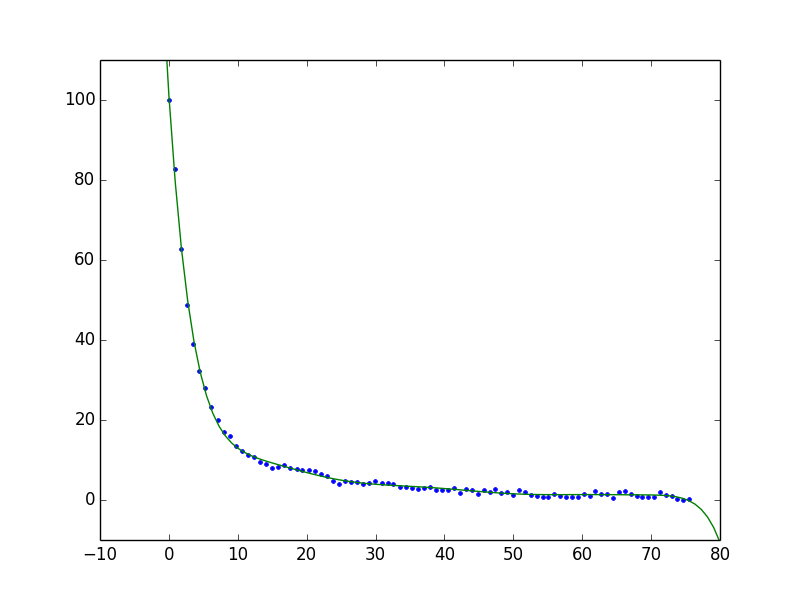
\includegraphics[height=140px]{img/regrD}
  \caption{Regression functions based on the samples.}
  \label{fig:regr}
\end{figure}


The speed of light transmission depends in primis on the speed at which the light itself can be turned on and off.
Figure \ref{fig:warmup} shows the warmup and cool down times for the low power LED over multiple instances, meaning the time that it takes for turning the light completely on from completely off, and vice versa.
These measurements depend on the reception rate of the system, which will be discussed in section \ref{recrates}.
A polynomial regression of 9th grade has been applied to the values in order to approximate the intermediate stages between the sample interval as well.
Fig. \ref{fig:regr} shows the regression functions and the sample points from which they originates, for one of the measurements.
For each curve, 10 measurements have been performed and approximated.
Table \ref{tab:warmup} shows the times for the LED to switch between specific brightness levels, as an average of every measurement.
Each row represents the time to reach the level on each column, for example the first row represents the time to reach any brightness level starting from 0\% brightness.
The table works both ways, in the sense that it shows the time for the warmup as well as the time for the cool down of the LED.
Warmup times are to the right side of the diagonal, while cool down times are on the left side.
The last row shows how long it takes to reach any level from a completely ON state, meaning starting from 100\% of brightness.

\begin{table}[hbt]
\centering
  \begin{tabular}{ l | c c c c c c c c c c c}
    & 0\% & 10\% & 20\% & 30\% & 40\% & 50\% & 60\% & 70\% & 80\% & 90\% & 100\% \\
    \hline
0\% & - & 0.3 & 0.66 & 1.08 & 1.52 & 2.12 & 2.82 & 3.78 & 5.38 & 10.4 & 50.66 \\
10\% & 55.88 & - & 0.36 & 0.78 & 1.22 & 1.82 & 2.52 & 3.48 & 5.08 & 10.1 & 50.36 \\
20\% & 61.86 & 5.98 & - & 0.42 & 0.86 & 1.46 & 2.16 & 3.12 & 4.72 & 9.74 & 50.0 \\
30\% & 63.76 & 7.88 & 1.9 & - & 0.44 & 1.04 & 1.74 & 2.7 & 4.3 & 9.32 & 49.58 \\
40\% & 64.9 & 9.02 & 3.04 & 1.14 & - & 0.6 & 1.3 & 2.26 & 3.86 & 8.88 & 49.14 \\
50\% & 65.76 & 9.88 & 3.9 & 2.0 & 0.86 & - & 0.7 & 1.66 & 3.26 & 8.28 & 48.54 \\
60\% & 66.4 & 10.52 & 4.54 & 2.64 & 1.5 & 0.64 & - & 0.96 & 2.56 & 7.58 & 47.84 \\
70\% & 66.98 & 11.1 & 5.12 & 3.22 & 2.08 & 1.22 & 0.58 & - & 1.6 & 6.62 & 46.88 \\
80\% & 67.48 & 11.6 & 5.62 & 3.72 & 2.58 & 1.72 & 1.08 & 0.5 & - & 5.02 & 45.28 \\
90\% & 67.92 & 12.04 & 6.06 & 4.16 & 3.02 & 2.16 & 1.52 & 0.94 & 0.44 & - & 40.26 \\
100\% & 68.28 & 12.4 & 6.42 & 4.52 & 3.38 & 2.52 & 1.88 & 1.3 & 0.8 & 0.36 & - \\
  \end{tabular}
  \centering
  \caption{Warmup times in [ms] of the LED, for specific levels of brightness. Row: from brightness, Column: to brightness.}
  \label{tab:warmup}
\end{table}

From the table as well as from fig. \ref{fig:warmup}, it can be seen that the LED is slightly faster at being turned on rather than off.
Also pretty indicative is the fact that about 90\% of the time used for turning a LED completely on or completely off, is spent to make a variation in the last 20\% of brightness levels, which means that a LED can reach a reasonably high brightness in a time relatively small compared to the full state change.
Interesting for later sections is that 50\% of the brightness can be reached in about 2 ms.

%distance
\subsection{Distance}
\label{distancephy}
Another factor that might affect the communication over light is the distance between emitter and sensor, closely bound with the brightness reachable from the light emitter and the presence and weight of light interference.
Intuitively, brighter lights will be visible from farther.
A low power LED cannot reach high levels of brightness, therefore it won't be visible at long distances.
Table \ref{tab:distancesphy} shows the results of different measurements taken at increasing distances sensor to light source.
Two different light sources have been tested, the low power (5V) LED and a commercial LED bulb powered by mains electricity (240V).
The reference for maximum brightness is achieved with a distance of 0 cm between receiver and light source, with the two nearly touching, represented as a 100\% of brightness.
Figure \ref{fig:distancephy} shows the measurements of the same experiments in a graphical manner, only for the low power LED.
In the figure, each colour represents a different distance, and each peak a different experiment.
The experiment was performed in a dark environment, minimising interference from other light sources.

\begin{table}[hbt]
\centering
  \begin{tabular}{c | c || c}
    distance & max. brightness LED & max. brightness bulb \\
    \hline
    0 cm & 100\% & 100\% \\
    10 cm & 42.81\% & 73.31\%\\
    20 cm & 14.28\% & 53.59\%\\
    30 cm & 8.57\% & 40.60\%\\
    40 cm & 5.00\% &31.55\%\\
    50 cm & 3.57\% & 25.03\%\\
    100 cm & 2.14\% & 10.27\%\\
    200 cm & - & 3.81\% \\
  \end{tabular}
 \caption{Maximum brightness over different distances.}
  \label{tab:distancesphy}
\end{table}

\begin{figure}[hbt]
	\centering
      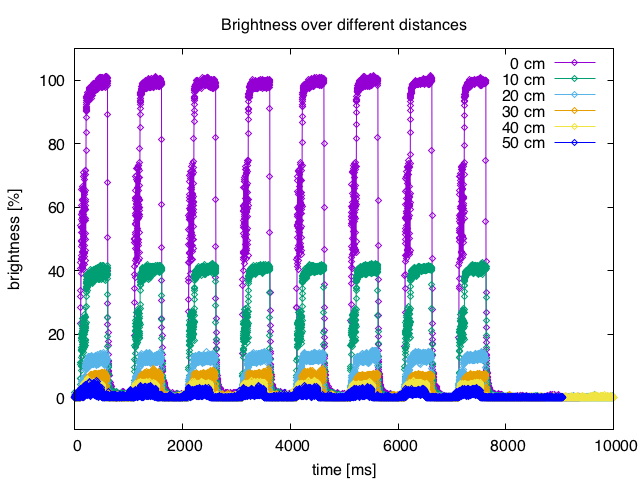
\includegraphics[height=180px]{img/distancephy}
  \caption{Brightness at different distances, low power LED.}
  \label{fig:distancephy}
\end{figure}

From the table and figure it can be seen that the maximum brightness registered from the sensor drops decidedly with increasing distance.
This obviously makes reliable communication over long distances harder.
The comparison between the two light sources clarifies the role of brightness in achieving certain distances.
The LED bulb has registered a brightness 5 to 6 times more intense than the low power LED, has a wider viewing angle and clearly is able to reach longer distances, about 4 times more than the single LED.\\
Another important implication with this results is the role of noise in the reception, both instrumental and environmental.
In the figure, noise can be graphically implied as the thickness of the lines.
Noise doesn't scale with the communication, meaning that if the maximum brightness perceived at a certain distance is 50\% of the brightness at 0 distance, the noise in this first case is not 50\% of the one used for reference, but stays constant.
This means that the lower the variation perceived, the more noise will play a role in the communication.
A remark on the experiments performed is that both lights used for testing are directional, with an optimal viewing angle of about 30$^{\circ}$ from the centre of the emitter for the LED and 120$^{\circ}$ for the bulb. 
The receiver, at the different distances, was always placed in the optimal viewing point in relation to the light direction.


%ambient
\subsection{Interference from ambient light}
Previous data about times to reach maximum brightness were measured in a condition of full darkness of the environment surrounding the light source, at minimal distance between transmitter and receiver.
But visible light communication is not necessarily used with this restrictions, it is in fact meant to be used over an open space, wirelessly,  meaning that interference from natural light or other light sources is very likely.
 Experiments have been performed to quantify the influence of ambient light on potential transmission.
 This is done by comparing the difference between the brightness measured by the sensor when the transmitter is turned on and the one when the transmitter is turned off.
 This represents the maximum potential amplitude of a signal.
 This difference will be measured without ambient light interference and used as a reference for the measurements that occur with ambient light interference.
 Since communication  will later rely on the quantification of light variations, it's important to establish if these variations will be substantially different with or without interference present.
 For these experiments, for ambient light it is meant light from any source that is not directed to the receiver but naturally permeates the environment surrounding the system.
 If the variation ON/OFF in a fully dark environment is represented as 100\%, the experiment shows that this difference is between 100\% and 120\% when ambient light is present, averaging at around 110\%. 
These measurements were taken at 0 distance and with direct exposure.
This increase could be explained with a higher sensibility of the sensor when exposed to higher levels of base brightness.
This suggests that ambient light interference doesn't affect transmission quality, at least in optimal conditions, with limited ambient light with no direct source pointing at the sensor and without accounting for distance.
Introducing distance as a parameter though, it appears that light intensity decreases faster over distance when in presence of other light sources.
Table \ref{tab:distancesphyINT} shows the results of testing the maximum brightness received over different distances, with presence of natural light.
The source of the ambient light does not face the sensor directly for these measurements.
The table also compares the results of the same tests performed in a completely dark environment.
Figure \ref{fig:distanchephyINT} shows the same results graphically.

\begin{table}[hbt]
\centering
  \begin{tabular}{c c l}
    distance & max. brightness, dark & max. brightness with natural light \\
    \hline
    0 cm & 100\% & 100\%\\
    10 cm & 42.81\% & 26.28\%\\
    20 cm & 14.28\% & 12.16\%\\
    30 cm & 8.57\% & 7.44\%\\
    40 cm & 5.00\% & 4.78\\
    50 cm & 3.57\% & 4.21\%\\
  \end{tabular}
 \caption{Maximum brightness over different distances, with interference from natural light.}
  \label{tab:distancesphyINT}
\end{table}

\begin{figure}[hbt]
\centering
  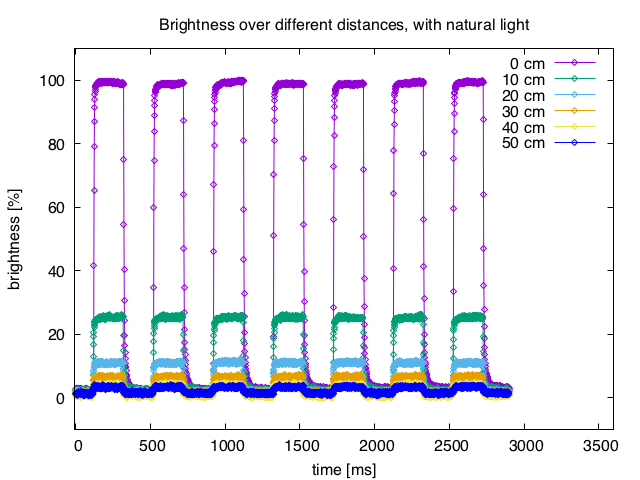
\includegraphics[height=180px]{img/distancephyINT}
  \caption{Brightness at different distances, low power LED with natural light interference.}
  \label{fig:distanchephyINT}
\end{figure}


%angle
\subsection{Angle}
In addition to the previous factors, also alignment between the light emitter and the light sensor might be of relevance when establishing communication between the two ends, under certain circumstances.
So far, in all of the communication tests performed on the system, the receiver was always in direct line of sight with the light emitter and centred to its focus.
However,  if the light source is directional or semi-directional, the angle of incidence would affect the ability of the sensor to register light variations.
This could also be the case for omni-directional light sources, when reflection of the light would be critical for it to reach the sensor.
For example, the light source could not be bright enough to reach reflecting surfaces or these could be absent.
In the case of a regular room as the location of the communication system,  the light source must be powerful enough to either reach the sensor directly with sufficient intensity, or to reach it indirectly by reflecting on the walls, ceilings or other surfaces.
Experiments have been performed with different angles to show how this factor affects overall reception with a directional light source.
The measurements have been taken at a distance of 10 cm between light source and sensor, in a otherwise dark environment.
\begin{table}[hbt]
\centering
  \begin{tabular}{c c}
    Angle & max.brightness \\
    \hline
    0$^{\circ}$ & 100\% \\
    40$^{\circ}$ & 60\% \\
    60$^{\circ}$ & 50\% 
  \end{tabular}
  \caption{Maximum brightness measured at different angles.}
  \label{tab:anglesphy}
\end{table}
These results suggest that the larger the angle of exposure, the less powerful the reception. 

\begin{figure}[hbt]
\centering
  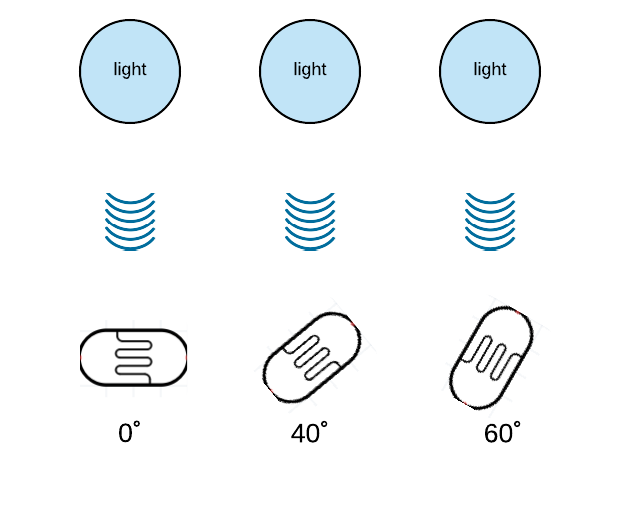
\includegraphics[height=140px]{img/angles}
  \caption{Sensor receiving light from the transmitter at different angles.}
  \label{fig:angles}
\end{figure}


%power ac vs dc
\subsection{Powerful lights and power source}
\label{acphy}
As can be deducted from the previous results, brighter and faster light sources are preferred to achieve better communication, preferably with an alignment between receiver and transmitter and no interference.
These are the optimal conditions for visible light communication. 
Sources that can turn on and off faster can potentially allow faster switching, which in turn allows faster communication.
Light sources that are brighter can be perceived at longer distances, and are less subject to interference.
Such lights have a higher power consumption than less performant ones.
If the vision is to have a smart environment with lights that serve the double purpose of lighting the environment for humans and transmit information to devices, the most natural thing would be to connect these lights to mains electricity like any other lamp.
This power source potentially allows the usage of much more powerful light bulbs then the low power LED used in the prototype.
In Europe, electric power supply for mains is of 230 V at a frequency of 50 Hz.
A distinctive trait of this power source is that it uses Alternating Current (AC).
Alternating current periodically reverses direction whereas direct current (DC) always flows in the same direction.
AC voltage can be expressed by a sinusoidal function, which means the current will vary its intensity in time.
Current will be higher near the peak, and lower near the time of the periodic switch in direction. 
This behaviour is clearly represented in figure \ref{fig:warmupAC}, when the light is ON after the warmup in the figure on the left, or before the cool down in the figure on the right.
The ON/OFF difference when measuring the light intensity with the receiver is over 500\% bigger than the LED of the prototype system, with similar rise speeds.
However, the fluctuations of AC during the ON state make it harder to use it for communication using On Off Keying, since that modulation scheme relies on variations in intensity.
A way around this would be to convert AC to DC with a process called rectification.
This involves the use of a capacitor connected between AC V$^{+}$ and Ground,  which lowers the amplitude of the AC significantly thus producing something very similar to DC.
Another problem to face however, as shown in the picture, is that these LED bulbs have a much slower fall time when switched off, which also would affect the switching frequency during transmission.

\begin{figure}[h]
\centering
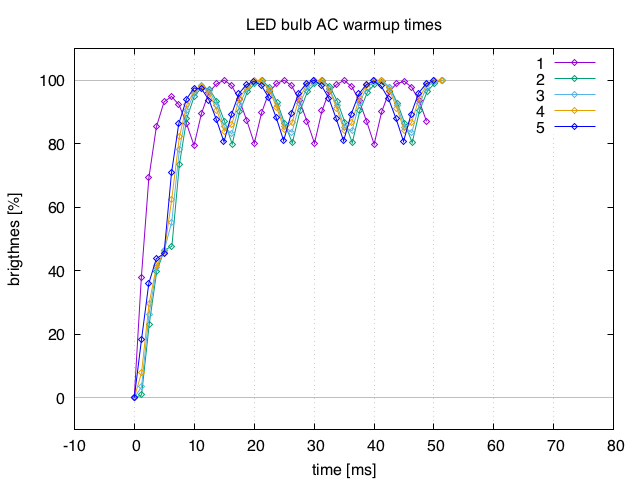
\includegraphics[height=140px]{img/warmup2}
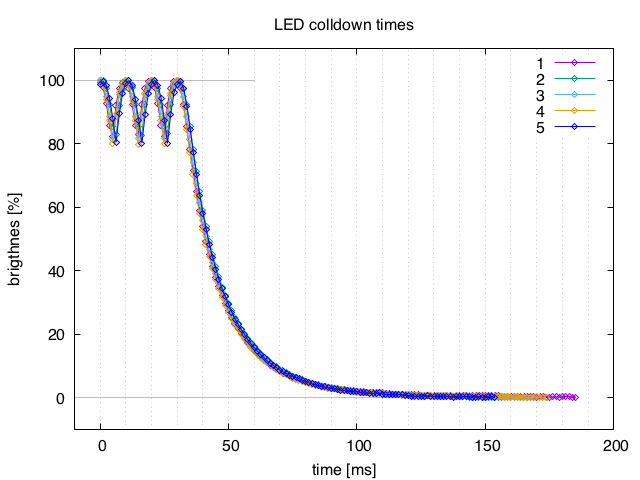
\includegraphics[height=140px]{img/warmdown2}
\caption{AC bulb warmup time, and phases of alternating current.}
\label{fig:warmupAC}
\end{figure}
